\documentclass{beamer}
\usetheme{Madrid}
\usecolortheme{default}

\title[Social Connections Analysis]
{Effects of Socialization on Mental Health}

\subtitle{STA130 Course Project}

\author[STA130] % (optional, for multiple authors)
{Edie Chen$^1$ \and Jason Li \and Zain Mahmoud \and Rana Nagash\\
TA: Oliver Gatalo\\
Professor Scott Schwartz}

\institute[UofT] % (optional)
{
  STA130: An Introduction to Statistical Reasoning and Data Science\\
  Department of Statistical Sciences\\
  University of Toronto
}

\date[November 2024] % (optional)


\logo{
\includegraphics[height=0.8cm]{logo_uoft}}

\definecolor{uoftblue}{RGB}{6,41,88}
\setbeamercolor{titlelike}{bg=uoftblue}
\setbeamerfont{title}{series=\bfseries}

\begin{document}

\frame{\titlepage}


\section{Introduction}

\begin{frame}
\frametitle{Introduction}
Social interactions play a pivotal role in shaping individual mental health outcomes. It is becoming increasingly easier, especially for teenagers, to connect with their friends virtually from the comfort of their homes. One may argue that this is harmful for their mental health; is this always the case?\\
Through this research, we aim to highlight the difference between physically interacting with community members as opposed to virtually connecting with them. \alert{Canadian Social Connections Survey (CSCS)} to investigate the relationship between various forms of social interactions (physical and non-physical) and how they affect the individuals' mental health states. 
This presentation outlines the variables we're using, our hypotheses, analyses, key findings, and the conclusions we've drawn from these findings.
In this study, we analyze data from the 
\end{frame}


\section{Research questions}

\begin{frame}
\frametitle{Our research questions}

\begin{block}{Question 1}
Do the frequency days where an individual spends at least 5 minutes physically socializing lessen an individual’s degree of depression?
\end{block}

\begin{alertblock}{Important theorem}
Does playing online games affect how often you feel depressed, and does going outside with friends counter-act that? 
\end{alertblock}

\begin{block}{Question 3}
    Does video chatting with others make one feel less lonely than text messaging? 
\end{block}
\end{frame}
\section{Question 1}
\begin{frame}
\frametitle{Question 1: Variables}
Independent variables:\\
CONNECTION\_social\_days\_family\_p7d\_grouped: days where individuals spent at least 5 minutes socializing with family.
CONNECTION\_social\_days\_friends\_p7d\_grouped: days where individuals spent at least 5 minutes socializing with friends.
CONNECTION\_social\_days\_coworkers\_and\_classmates\_p7d\_grouped: days where individuals spent at least 5 minutes socializing with co-workers or classmates.
CONNECTION\_social\_days\_neighbours\_p7d\_grouped: days where individuals spent at least 5 minutes socializing with neighbours.
Dependent variables:\\
WELLNESS\_phq\_score: metric used to characterize an individual's level of depression on a scale of 0-6.\\
\end{frame}


\begin{frame}{Preliminary analysis}
    After keeping only the columns we're interested in and cleaning the data, we were left with 575 rows and 6 columns.
\begin{figure}
    \centering
    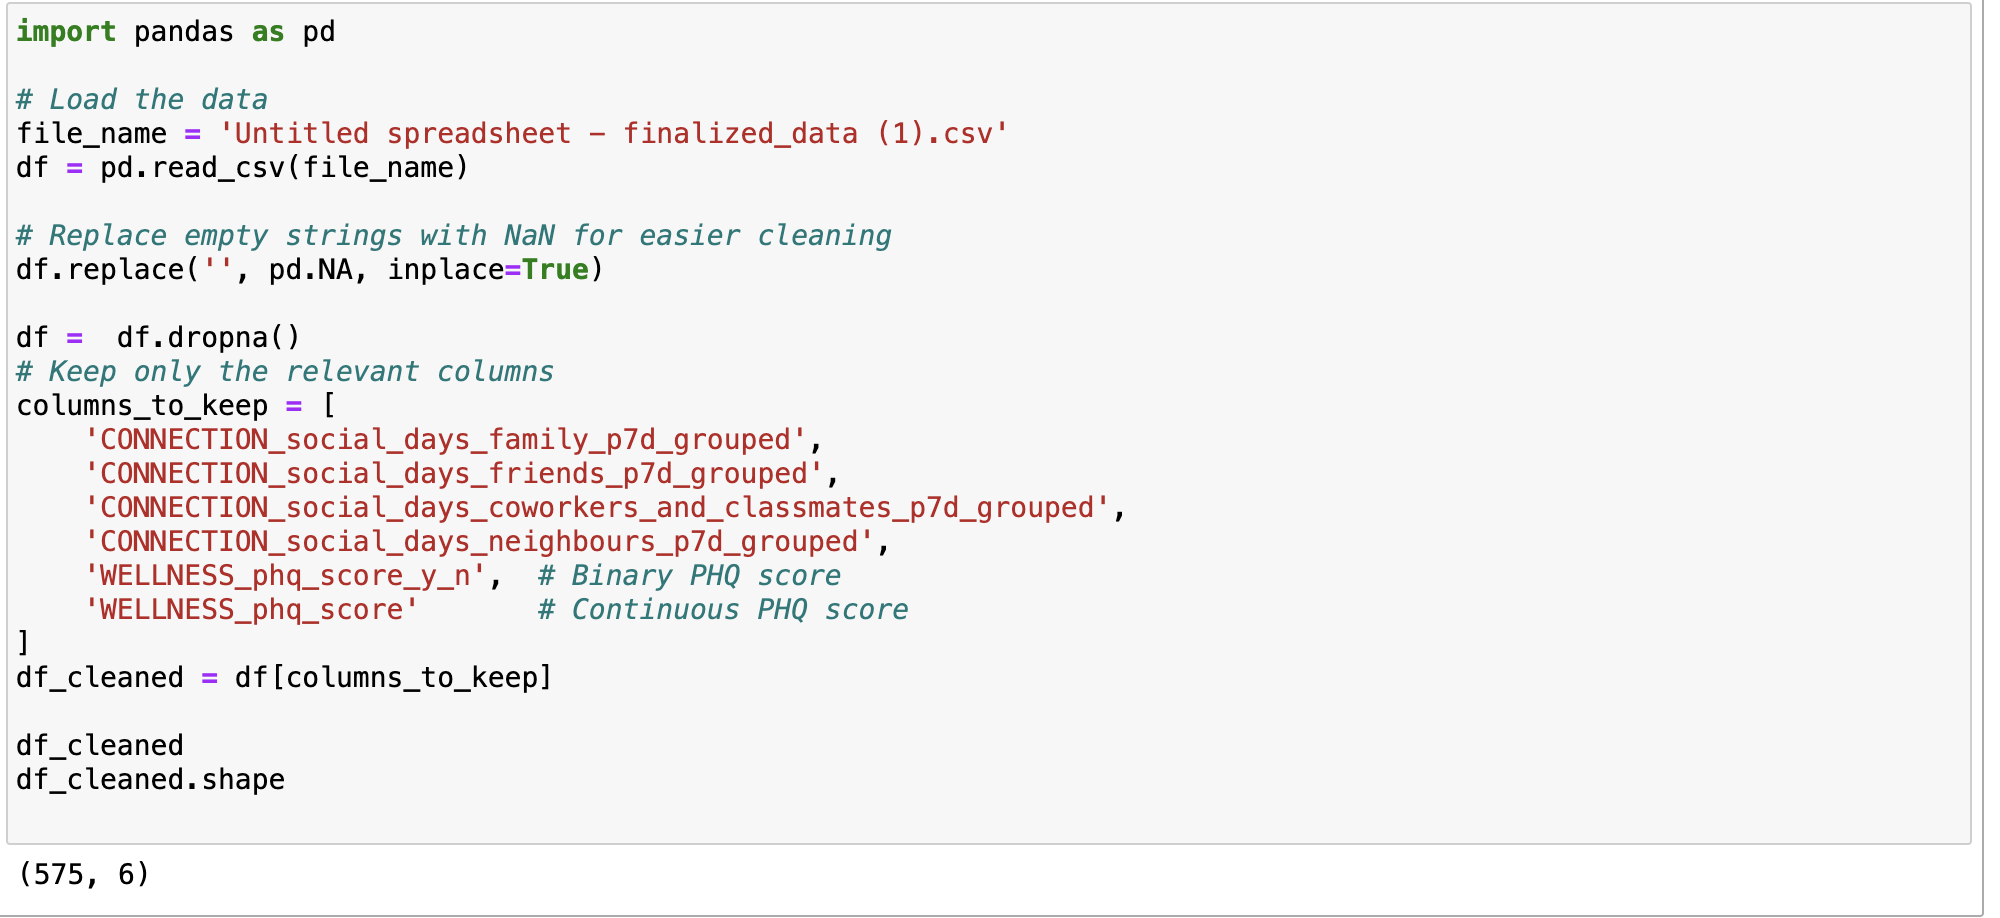
\includegraphics[width=1\linewidth]{image.png}
    \caption{6x575 cleaned dataframe}
    \label{fig:enter-label}
\end{figure}
\end{frame}

\begin{frame}{Preliminary analysis}
    The independent variables were categorical with 4 categories each: 
\begin{figure}
    \centering
    
\includegraphics[width=1\linewidth]{image2.png}
    \caption{Unique data entries in one of the columns }
    \end{figure}
    To better analyze the data, we gave each category a numeric value based on the midpoint of the interval. For example, the 'Most days (4-6)' category was assigned 5 (representing the midpoint of the number of days). Then, we added another column to represent the total number of days where each individual spent at least 5 minutes socializing with any one of the groups above using the numeric values we assigned to each category. 
\end{frame}


\begin{frame}{Analysis}
    First, we examined the relationship between the total column and the numeric PHQ score column. We did this by fitting a simple linear regression through the data.
    \begin{columns}
        \column{0.5\textwidth}
        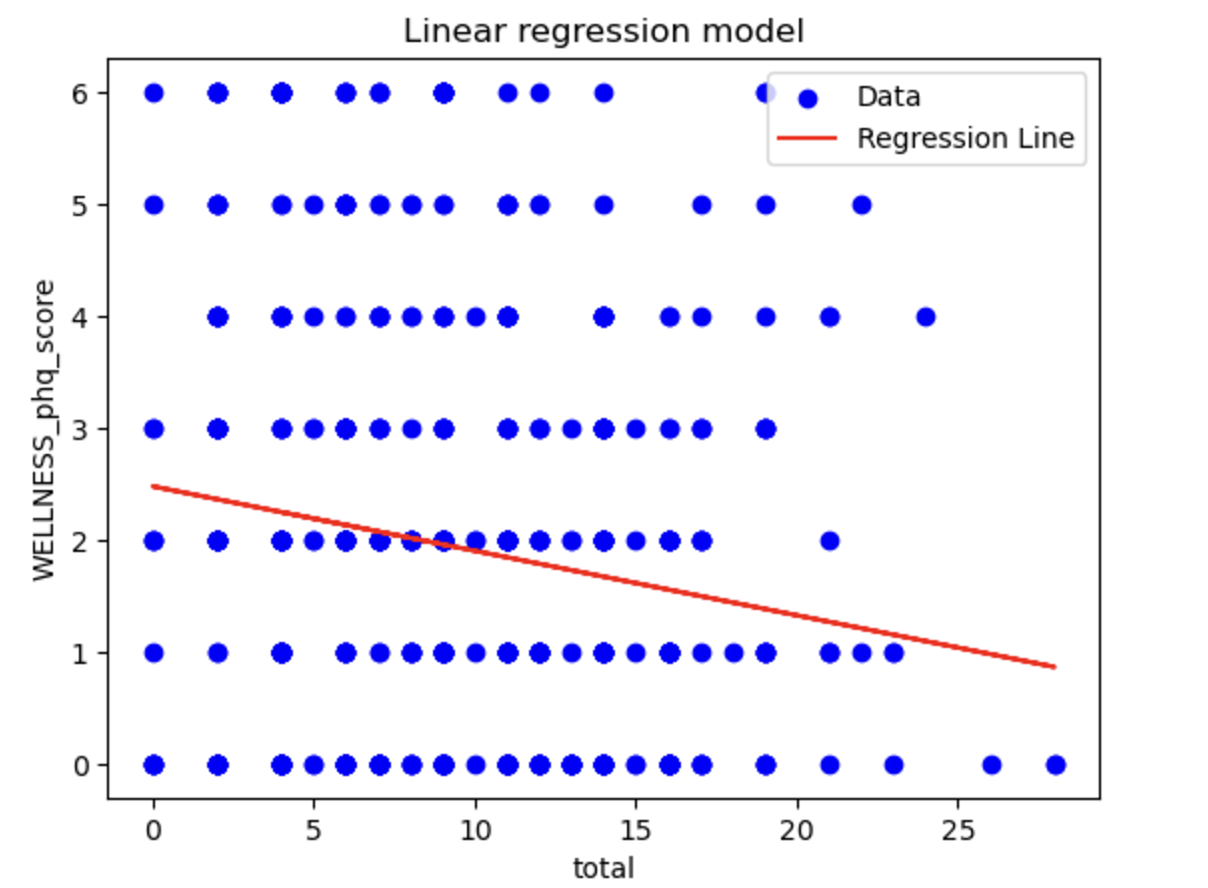
\includegraphics[width=1\linewidth]{model1.png}\\
        \column{0.5\textwidth}
        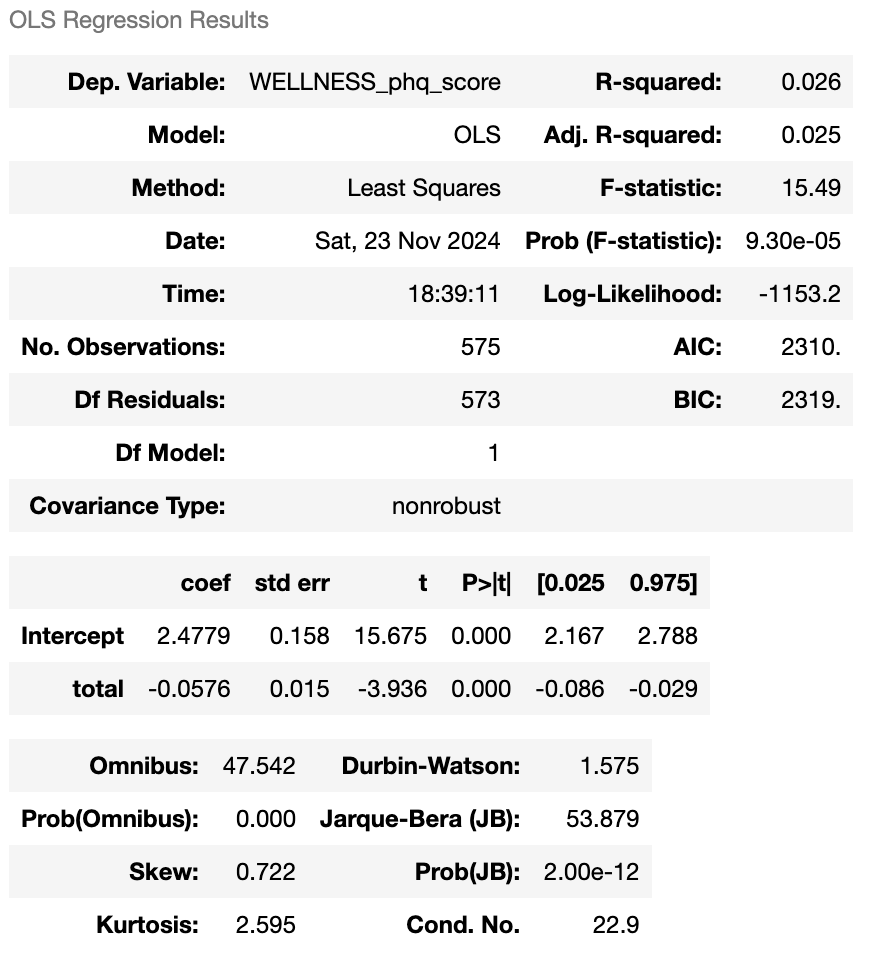
\includegraphics[width=1\linewidth]{summarystats.png}

        
    \end{columns}
\end{frame}

\begin{frame}{Analysis}
    We then created a bootstrapped distribution of model slope coefficients by repeatedly resampling from our original sample and refitting OLS models through the samples. Then, we created a 95\% confidence interval of our bootstrapped coefficients for inference.
    \begin{figure}
        \centering
        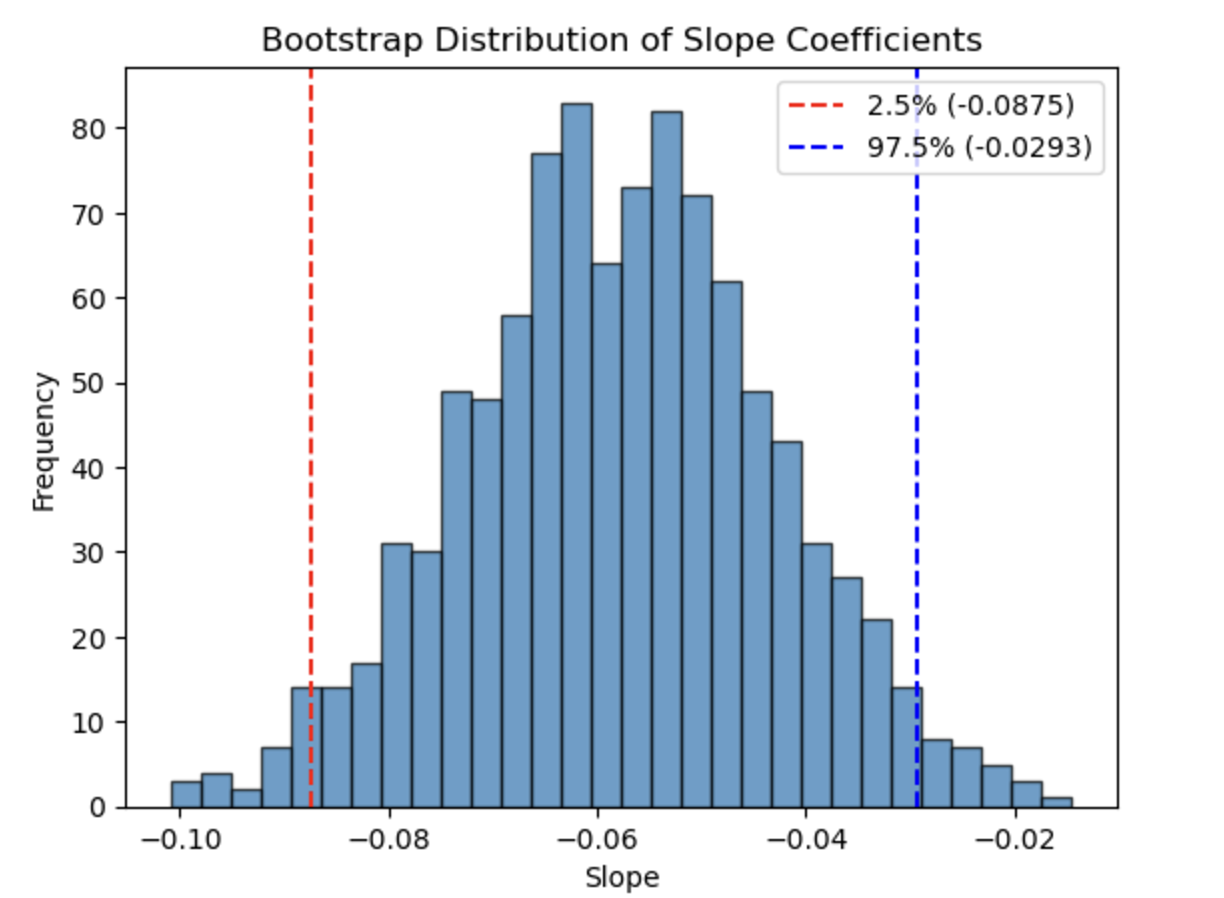
\includegraphics[width=0.5\linewidth]{95CI.png}
        \caption{95\% confidence interval}
        \label{fig:enter-label}
    \end{figure}
\end{frame}

\begin{frame}{Summary and conclusion}
The confidence interval we constructed only contained negative slopes between $-0.0875$ and $-0.0293$ and so we can conclude with 95\% confidence that the true value of the slope coefficient lies in that interval. This means that as the number of days where an individual spends at least 5 minutes socializing increases, the average depression score decreases. However, the values of the slopes are very small and so the effect of socializing on depression scores is minuscule (albeit negative).
    
\end{frame}


\section{Question 2}
%ADD YOUR FRAMES BELOW
\begin{frame}{Frame Title}

\end{frame}


\section{Question 3}
%ADD YOUR FRAMES BELOW
\begin{frame}{Frame Title}
    
\end{frame}

\end{document}